\documentclass[aip, jcp, reprint, twocolumn]{revtex4-2}

\bibliographystyle{apsrev4-2}

\usepackage{physics}
\usepackage{amsmath}
\usepackage{amssymb}
\usepackage{mathtools}
\usepackage{graphicx}
\usepackage{dcolumn}
\usepackage[colorlinks=true, linkcolor=black, urlcolor=blue, citecolor=black, anchorcolor=black]{hyperref}

\graphicspath{{"figures/"}}
\begin{document}
%Title of paper
\title{Coherent Hyper-Raman Four Wave Mixing Vibrational Spectroscopy}


\author{Ryan P. McDonnell} 
\author{Daniel D. Kohler}
\author{John C. Wright} \email{wright@chem.wisc.edu}

\affiliation{Department of Chemistry, 
        University of Wisconsin - Madison, 
        Madison, Wisconsin 53706, 
        United States of America}

\date{\today}

\begin{abstract}
Nonlinear, four wave mixing vibrational spectroscopies are often used to probe intramolecular vibrational coupling and relaxation dynamics.
Three wave mixing vibrational spectroscopies are similarly used to understand the spectroscopy and dynamics of interfacial species.
Most of these methods rely on infrared or Raman transitions to generate output. 
Implementing a nonlinear spectroscopy involving hyper-Raman transitions, first appearing under third order perturbation theory, can provide a useful analogue to infrared and Raman based nonlinear spectroscopies to understand the spectroscopy and dynamics of isotropic systems.
Hyper Difference Frequency Generation (hyper-DFG, or HDFG) spectroscopy, also known as singly vibrationally enhanced spectroscopy (SIVE), is an underdeveloped, hyper-Raman based four wave mixing vibrational spectroscopy. 
The spectroscopic and dynamic properties of HDFG have not been fully explored.
We derive selection rules for singly resonant hyper-DFG and demonstrate it provides a simpler method to extract hyper-Raman polarizabilities ($\beta$).
HDFG output is shown to be similar in magnitude to vibrational sum frequency generation (vSFG). 
We demonstrate the properties and capabilities of HDFG through measuring spectra and coherence dynamics of multiple infrared active modes in CH$_3$CN.
HDFG shows promise as a method to disentangle ultrafast vibrational dynamics in isotropic systems without need for anharmonicities.

\end{abstract}

\maketitle

\section{Introduction}
Coherent multidimensional spectroscopy (CMDS) is a family of three and four wave mixing methods which form the optical analogue of multidimensional nuclear magnetic resonance (NMR) spectroscopy.\cite{RN103, Cho2008, RN335}
Multiresonant, four wave mixing CMDS experiments, first proposed by Oudar and Shen in 1980,\cite{RN307} directly probe coupling between different vibrational, electronic, and vibronic states. \cite{RN307, RN281, RN103, RN342, Cho2008, RN335, Ogilvie2019, RN325} 
CMDS has resolved anharmonicities and other intramolecular couplings in numerous systems. \cite{RN345, RN342, RN343, RN324, RN329, RN120, Czech2015, Gaynor2017, Ogilvie2019, RN325}
A particular class of CMDS methods, coherent Raman based four wave mixing spectroscopies, can provide explicit probes of these couplings in a variety of systems. \cite{RN103, RN335}

\begin{figure*}[!htbp]
	\centering
	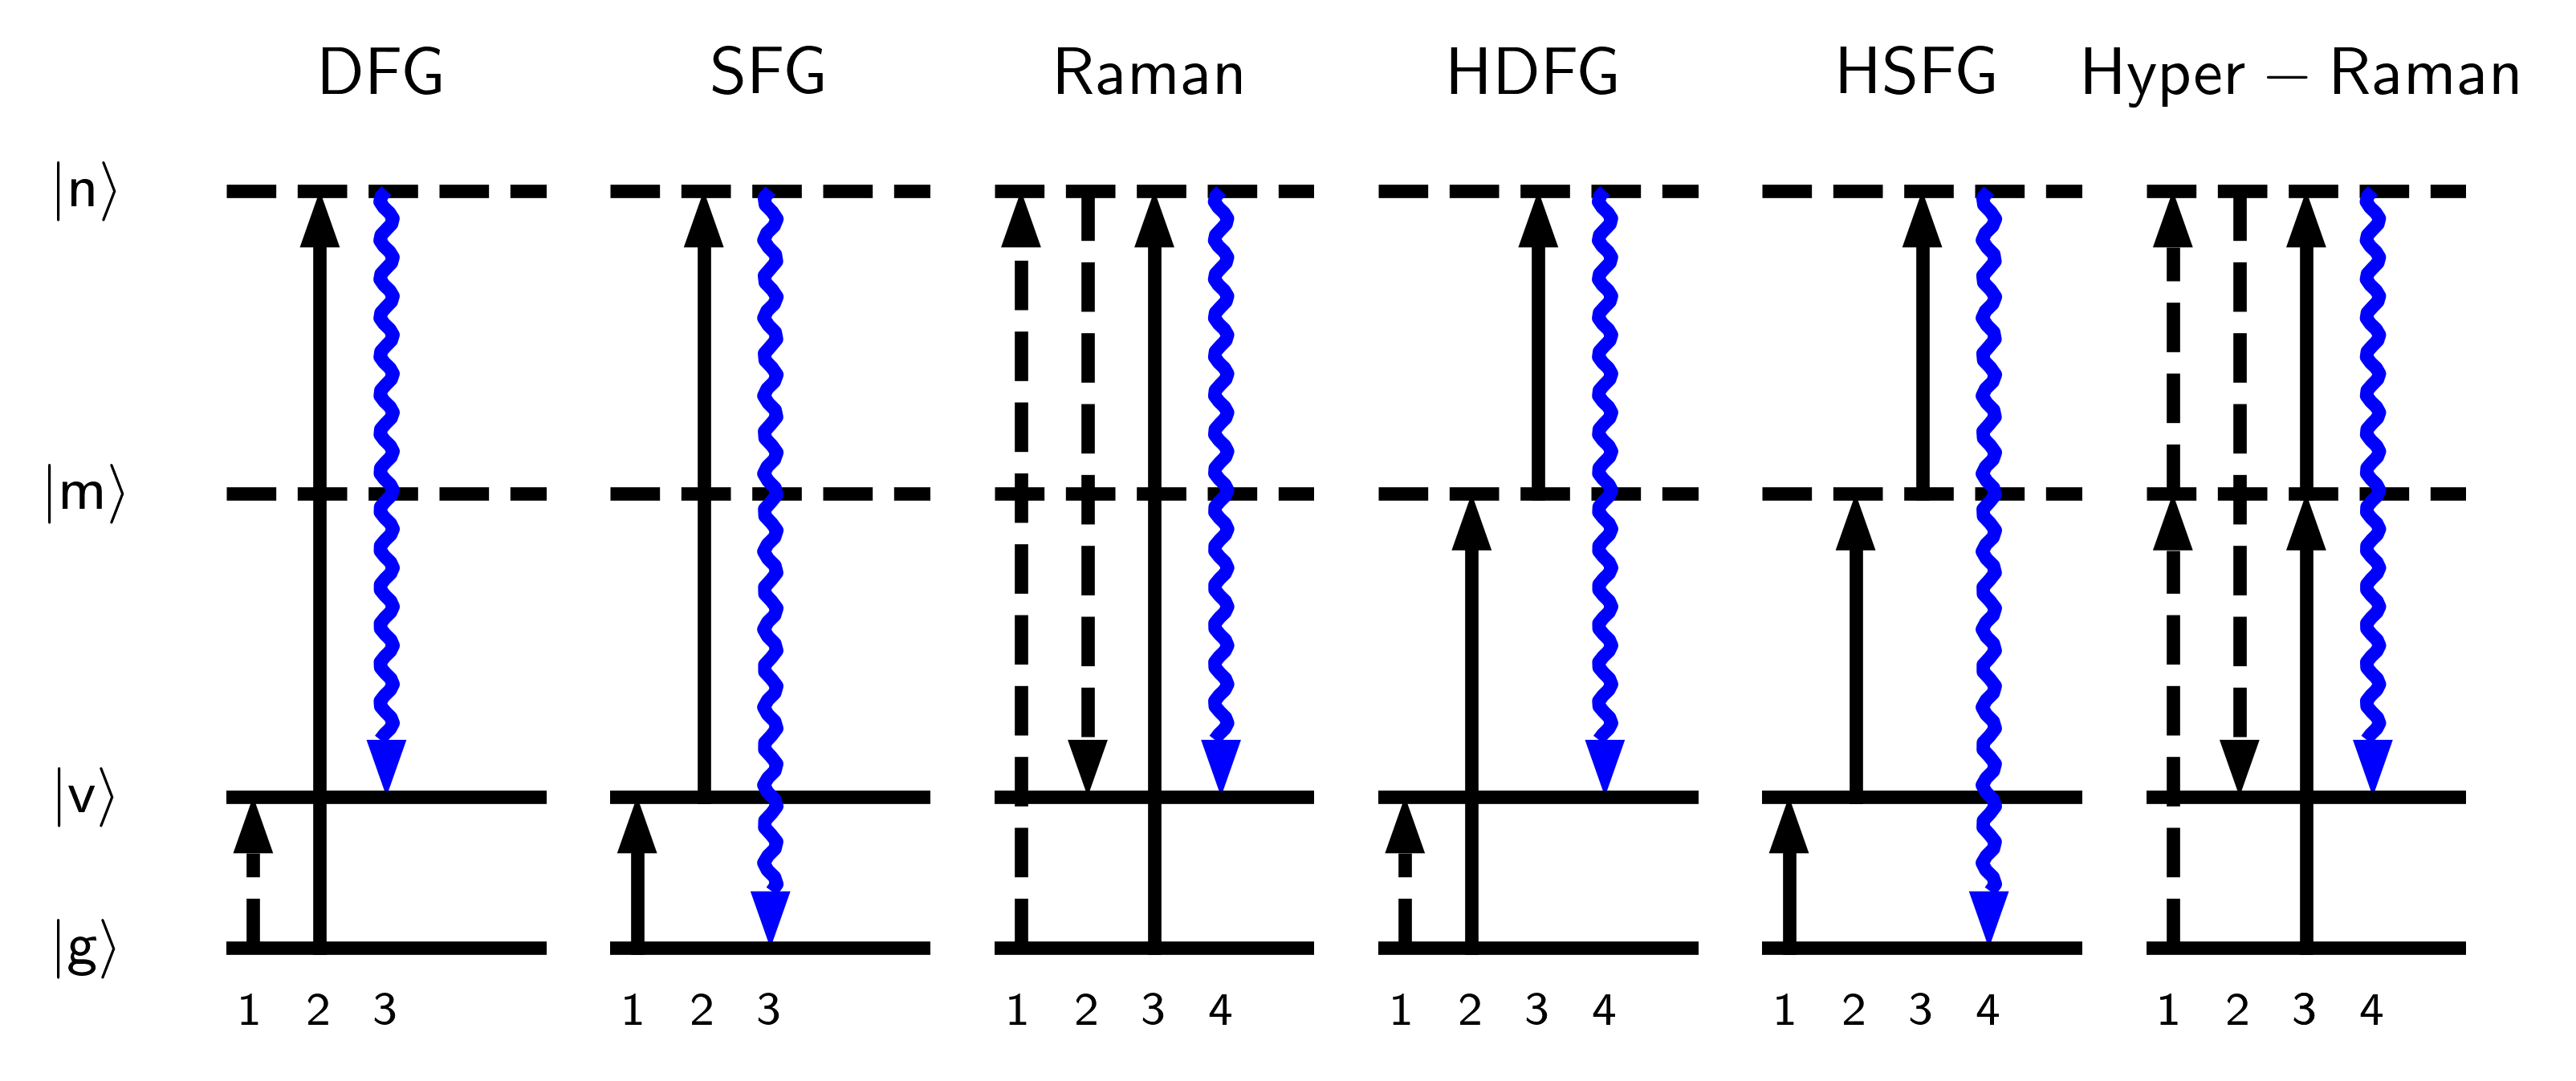
\includegraphics[width=6.66in]{comparisonwmel.png}
	\caption{Wave Mixing Energy Level (WMEL) diagrams of difference frequency generation (DFG), spontaneous Raman scattering, hyper difference frequency generation (HDFG) and spontaneous hyper-Raman scattering. \cite{RN286, RN352}
		$\ket{g}$ is the ground state, $\ket{v}$ is an infrared active vibration and $\ket{m}, \ket{n}$ are virtual states.
		Solid and dashed horizontal lines indicate real and virtual states, whereas solid and dotted arrows indicate ket and bra side transitions, respectively. 
		}
	\label{fig:comparisonwmel}
\end{figure*}

Not all CMDS methods are used to dissect intramolecular couplings.\cite{Shen1987_CPL}
The most well known example is sum frequency generation (SFG), a three wave mixing technique used to interpret vibrational structure and dynamics at interfaces. \cite{RN224, Piontek2023}
Non-parametric, hyper difference frequency generation (hyper-DFG, or HDFG) spectroscopy, similar to difference frequency generation (\autoref{fig:comparisonwmel}), is a four wave mixing method which, when detuned from  electronic resonances, does not probe intramolecular couplings. 
HDFG was the first infrared CMDS method to successfully discriminate against non-resonant background.\cite{RN351, RN352}
HDFG has also been referred to as singly vibrationally enhanced (SIVE) spectroscopy. \cite{RN351}
In HDFG, an infrared pulse is resonant with a vibrational mode, and two other input pulses are used to induce a scattering process to provide output.
HDFG was documented long ago to have characteristics similar to spontaneous hyper-Raman scattering spectroscopy. \cite{RN352}
Hyper-Raman scattering is the two photon analogue to Raman scattering. \cite{Cyvin1965, Terhune1965, Kozich2007}
Compared to Raman spectroscopy, hyper-Raman scattering cross sections are often small, making it a difficult technique to successfully implement.\cite{RN515, Kelley2010} 
The different selection rules of hyper-Raman scattering, however, make it a unique alternative to Raman scattering to understand vibrational spectra and vibronic coupling in molecular systems.
Some years ago, Cho et al. proposed parametric six wave mixing techniques as the coherent analogue of hyper-Raman scattering. \cite{Cho1997, Cho1998}
However, since most six wave mixing methods cascade into four wave mixing processes,\cite{RN243, Cho2000_Cascade}, and their output would be dependent upon the square magnitude of the hyper-Raman scattering cross section, a small number,\cite{RN515} it is preferable to investigate coherent four wave mixing analogues to hyper-Raman scattering.

While HDFG showed promise as an upconverted infrared spectroscopy method, it was quickly supplemented by a doubly vibrationally resonant method, doubly vibrationally enhanced (DOVE) spectroscopy, to investigate intra- and intermolecular vibrational coupling. \cite{RN345, RN101, Cho2000}
As a result, investigations of HDFG stagnated; to date, there are less than a dozen studies which report on HDFG. \cite{RN350, RN416, RN351, RN352, RN353, Chen1998, RN362, RN418, Bonn2024, McDonnell2024}
Recent reports highlight non-negligible HDFG interference in DOVE experiments as well as the suitability of HDFG pathways to interpret ultrafast relaxation dynamics in isotropic systems. \cite{Bonn2024, McDonnell2024}
These reports motivate deeper analysis on the properties of HDFG spectroscopy. 

Fully coherent, ultrafast probes of vibronic coupling would yield insight into processes that control ultrafast electronic relaxation in molecular and biological systems. \cite{Bredenbeck2015, Arsenault2021}
Some years ago, Cho proposed a parametric, doubly resonant infrared/visible pathway to probe vibronic coupling in isotropic systems. \cite{Cho2001}
In this method, a single infrared pulse is resonant with a vibrational mode, and a two photon absorption event from a near infrared (NIR) or visible pulse resonant with an electronic or vibronic state is used to generate the four wave mixing signal.
The non-parametric pathways similar to this method are referred to herein as doubly resonant HDFG (DR-HDFG).
Methods analogous to DR-HDFG, where two photon absorption from the infrared pulse and one photon absorption from the visible pulse is used to generate output, i.e., stimulated Raman processes, have been reported. \cite{RN301, RN120} 

An experimental complexity in executing Raman based four wave mixing experiments is the demand of three separate input pulses, often at different frequencies.
For example, in the case of DOVE, two of the three inputs must be scanable infrared pulses. \cite{RN345} 
Only recently have methods been developed for seamless tuning and scanning of ultrafast optical parametric amplifiers across swaths of frequency space. \cite{RN162, McDonnell2024, SkyeOPA, KyleOPA}
Since HDFG demands only a single resonance to be scanned, the experiment can be performed using two input pulses: one tunable, infrared OPA to scan across vibrational resonances, and a two photon absorption from the signal process of a separate OPA, or output from the oscillator which pumps the infrared OPA. \cite{Wang2021}
As such, laboratories experienced in sum frequency generation (SFG) spectroscopy can perform HDFG spectroscopy to understand bulk dynamics and spectroscopy using nearly the same setup.\cite{Shen1987_CPL}

Inspired by recent work which demonstrated the presence of HDFG in ultrafast DOVE experiments, we investigate the parameters which result in both SR and DR-SIVE output. \cite{Cho2000, Bonn2024, McDonnell2024}
This paper is outlined as follows.
In section \ref{steadystate}, we discuss the selection rules behind singly and doubly resonant HDFG first through the Placzek approximation, and then through hyper-Raman A,B,C coefficients.
In section \ref{quant}, the quantitative aspects of HDFG are discussed, and a method to extract hyper-Raman hyperpolarizabilities ($\beta_{ijk}$) from HDFG spectra is identified.
In section \ref{mixeddomain}, mixed time-frequency domain HDFG is discussed, and is applied to the simple case of CH$_3$CN in section \ref{Expt}. 

\section{Experimental}\label{experimental}
The ultrafast laser system has been described in detail elsewhere. \cite{RN278}
Briefly, an 80 MHz Ti-Sapphire ultrafast oscillator  (Spectra-Physics Tsunami) created 35 fs seed pulses, amplified by a 1 kHz regenerative amplifier (Spectra-Physics Spitfire Ace) to approximately 0.5 W.
A mask in the regenerative amplifier stretched the input pulses to roughly 1 ps.
The resultant output was used to pump four independent OPAs, two of which are relevant for this study.
OPA1 (TOPAS-800, Light Conversion), referred to as $\omega_1$, was tuned for difference frequency generation (DFG) with an external stage (NDFG ``DF2'', Light Conversion).
OPA2 (OPA-800C, Spectra Physics), referred to as $\omega_2$, was tuned in its signal arrangement. 
OPA3, a homebuilt OPA, is tuned in its signal arrangement and referred to as $\omega_3$.
Grating and crystal positions in OPA1 was externally controlled using \texttt{WinTOPAS} (Light Conversion).
Grating and BBO crystal positions in OPA2 and OPA3 were computer controlled through communication with DC actuators.
The OPAs were independently tuned through the \texttt{Attune} package, controlled by the \texttt{yaqc} and \texttt{Bluesky} packages. \cite{RN414, RN386, SkyeOPA, KyleOPA}
The power spectra and tuning results are found in Figure X. %todo: actually graph these
Movable retroreflectors (Thorlabs) controlled by 50 mm DC actuators (PMC) are used to measure coherence dynamics.
The beams are focused using a BOXCARS geometry.\cite{RN308, Kaufman2024}
To enforce frequency dependent temporal pulse overlap, the maximum points of a third order cross correlation between $\omega_1$ and $\omega_3$ measured in CaF$_2$ were used to generate frequency dependent zero delay values.
The nonlinear output was isolated through chopping schemes and a set of spatial apertures, directed into a monochromator (Horiba Micro-HR) and homodyne detected through a photomultiplier tube (Hamamatsu H7422-20), recorded and converted to digital output using a data acquisition unit (National Instruments).
\textit{in-situ} power corrections are performed by dividing the recorded spectra by OPA output measured by home-built pyroelectric detectors.
All spectra are reported on the intensity scale.

The cyanocobalamin (CNCbl) [DOT Scientific inc., CAS no. 68-19-9] samples were prepared as drop casted thin films.
CNCbl was dissolved in methanol (MeOH) [Fisher Scientific, HPLC Grade, CAS no. 67-56-1] until a concentrated solution was formed (concentration $\sim$ 10 mg CNCbl/ mL MeOH). 
All chemicals were used as obtained without further purification.
The solution was deposited on a microscope coverslip and allowed to dry in a dessicator until a thin layer was formed.

\section{Steady State HDFG Spectroscopy}\label{steadystate}
\subsection{Placzek Method}
Singly resonant hyper difference generation spectroscopy (HDFG) spectroscopy has potential to provide deeper insight into single quantum decoherence times and molecular orientation in condensed systems.
Similarities between HDFG spectroscopy, infrared spectroscopy and spontaneous hyper-Raman scattering have been noted previously. \cite{RN352, Bonn2024, McDonnell2024}
In this section, we investigate the steady state properties of HDFG and make the connections between HDFG and hyper-Raman scattering explicit.

It is useful to expose relationships between transition dipoles, Raman polarizabilities and hyper-Raman hyperpolarizabilities in the driven limit. \cite{Druet1978, Simpson2004}
In the driven limit, under the electric dipole approximation, the I$^{th}$ component of the third order nonlinear output polarization, ${P}^{(3)}_I$, of any four wave mixing process, induced by electric fields E, at output frequency $\omega_4$ is written as (using Einstein summation) \cite{RN307}
\begin{equation} \label{polarization}
{P}^{(3)}_I (\omega_4)  = \chi^{(3)}_{IJKL} E_J E_K E_L 
\end{equation}
where $\chi^{(3)}_{IJKL}$ is the IJKL element of the third order electrical susceptibility, a rank four tensor, generally written as
\begin{equation}
	\chi^{(3)}_{IJKL} = NF(\omega_4) \langle \gamma_{ijkl} \rangle
\end{equation}
where N is a number density, F is the Lorentz local field factor, and $\gamma_{ijkl}$ is the third order polarizability (i.e., second hyperpolarizability). 
The brackets indicate an orientational average. 
Uppercase letters refer to laboratory frame coordinates and lower case letters refer to molecular frame coordinates.

To make the connection between HDFG and hyper-Raman scattering, we investigate its gross selection rules.
By propagating density matrix elements in the steady state limit, the HDFG hyperpolarizability is \cite{RN119}
\begin{equation}\label{sivegamma}
		\gamma_{ijkl} =	- \sum_{m, n} \frac{1}{\varepsilon_0} \frac{1}{4D} \frac{1}{\hbar^3} \frac{\mu^{vn}_{i} \mu^{nm}_{j} \mu^{mg}_{k} \mu^{gv}_{l} }{\Delta_{nv} \Delta_{mv}\Delta_{gv}}  \rho_{gg}
\end{equation}
where: $\mu^{ab}_{j}$ is the $j^{th}$ element of $\mel{a}{\vec{\mu}}{b}$, $\Delta_{kl} = \omega_{kl} - \omega_{j} - i\Gamma_{kl}$, $\omega_j$ is the frequency of the j$^{th}$ input field, $\Gamma_{kl}$ is the dephasing of $\rho_{kl}$ and $\rho_{gg}$ is the ground state population.
D, the Maker-Terhune degeneracy factor, accounts for permutation symmetry in $\gamma_{ijkl}$.\cite{RN134} 
For a HDFG experiment using two or three distinct input fields, as considered here, D = 6.
We first investigate the selection rules through a Placzek type formalism.
Contracting over the virtual states forms the hyper-Raman hyperpolarizability $\beta$.\cite{Long1970} 
Assuming $\omega_2$, $\omega_3$ are significantly detuned from any local resonance (\autoref{fig:comparisonwmel}),\cite{Placzek1934, Long1970} \autoref{sivegamma} is written as 
\begin{equation}\label{sivebeta}
	\gamma_{ijkl} =	-\frac{1}{\varepsilon_0} \frac{1}{24 \hbar}\frac{\beta^{gv}_{ijk} \mu^{gv}_{l}}{\Delta_{gv}} \rho_{gg}
\end{equation}
It is important to note that the properties of $\beta_{ijk}$ change dependent upon whether $\omega_2$ and $\omega_3$ are degenerate. \cite{Andrews1978, Altmann1982}
Taylor expanding the dipole and first hyperpolarizability operators in terms of an n$^{\text{th}}$ normal mode coordinate $Q_n$ about equilibrium as\cite{Long1970}
\begin{subequations}
	\begin{equation}
		\mu = \mu_0 + \frac{\partial \mu}{\partial Q_n} Q_n + \order{{Q_m Q_n}}
	\end{equation}
	\begin{equation}
		\beta = \beta_{0} + \frac{\partial \beta}{\partial Q_n} Q_n + \order{{Q_m Q_n}}
	\end{equation}
\end{subequations}
and substituting into \autoref{sivebeta} gives the HDFG hyperpolarizability to $\order{Q_n}$ as \begin{equation}\label{SIVEselection}
	\gamma_{ijkl} =	-\frac{1}{\varepsilon_0} \frac{1}{48 m_n \omega_{vg}}  \frac{1}{{\Delta_{gv}}} \ \frac{\partial \beta^{gv}_{ijk}}{\partial Q_n} {\frac{\partial \mu^{gv}_{l}}{\partial Q_n}}  \rho_{gg}
\end{equation}
where $\mel{v}{Q_n}{g} = \sqrt{\frac{\hbar}{2m_n\omega_{vg}}}$ and $m_n$ is the ``mass'' of the $Q_n$ mode.  \cite{RN230}
Since this expression is non-zero in the harmonic oscillator limit, HDFG output is allowed for harmonic transitions. 
Similar to SFG, HDFG does not demand anharmonic ground state potential energy surfaces for spectral output. \cite{Shen94, Cho2000}
This selection rule is generally valid for any HDFG or hyper sum frequency generation (HSFG) process in the $-\vec{k}_1 + \vec{k}_2  + \vec{k}_3$ and $\vec{k}_1 + \vec{k}_2  + \vec{k}_3$ phasematching geometries when $\omega_2$ and $\omega_3$ are sufficiently detuned from any resonance.

\begin{figure}[!htbp]
	\centering
	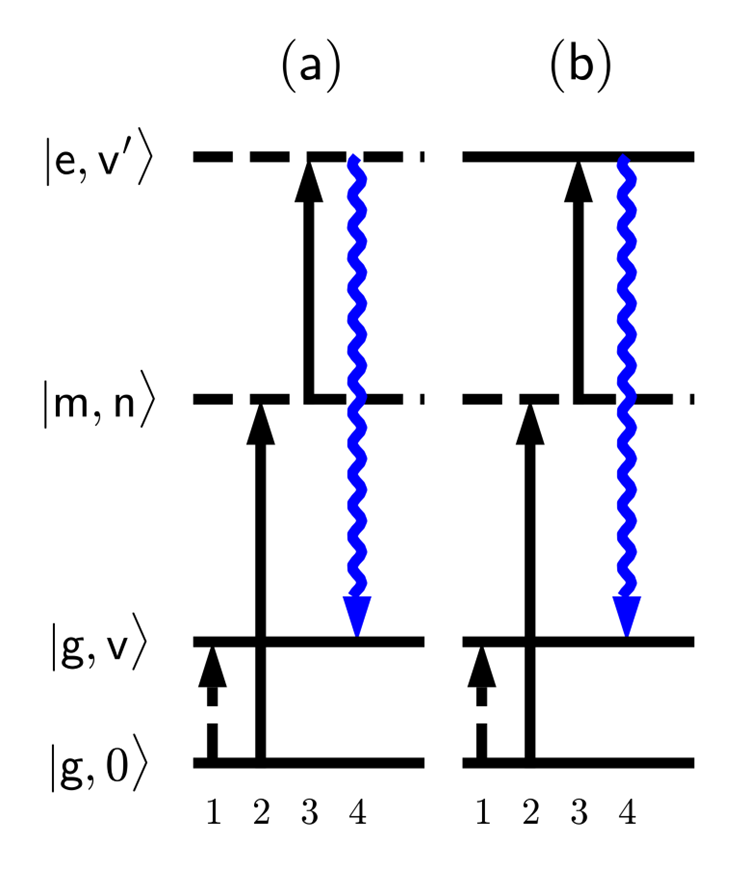
\includegraphics[width=3.375in]{hdfg.png}
	\caption{WMEL diagrams of (a) singly resonant and (b) doubly resonant HDFG. 
	}
	\label{fig:hdfg}
\end{figure}
\subsection{Albrecht Type Expansion}
While Placzek type arguments provide the general source of HDFG output, it is insightful to interpret the origin of signal in terms of Albrecht ABC type terms.\cite{Ziegler1988} 
We write $\beta_{ijk}$ in \autoref{SIVEselection} using the hyper-Raman ABC formalism to understand how vibronic coupling manipulates selection rules for singly and doubly resonant HDFG (\autoref{fig:hdfg}). \cite{Ziegler1988, Baranov1990}
To employ this formalism, we write the states in terms of a Born-Oppenheimer basis $\ket{a,b}$, where $\ket{a,b} = |a(Q)) \otimes \ket{b}$ for electronic states $\{|a(Q))\}$ and vibrational states $\{\ket{b}\}$ (i.e., adiabatic approximation). \cite{BornOppenheimer, Tang1970}
The dependence of the electronic states on the adiabatic parameter $Q$ is suppressed for simplicity.
The states are labeled as shown in \autoref{fig:hdfg}.
For consistency with previous reports, we use $\vec{R}$ to denote electric transition dipole moments ($\vec{\mu}$ is reserved for transitions between states on the ground electronic state). \cite{Tang1970}
Following the approach which gave \autoref{sivegamma}, we find
\begin{equation}\label{drgamma_notaylor}
	\gamma_{ijkl} = -\frac{1}{\varepsilon_0} \frac{1}{24 \hbar^3} \sum_{m,n,e,v'} \frac{
		R_{i}^{gv, ev'} 
		R_{j}^{ev',mn} 
		R_{k}^{mn,g0} 
		R_{l}^{g0,gv} 
	}{\Delta_{g0,gv}
		\Delta_{ev', mn}
		\Delta_{mn, g0}
	}
\end{equation}
where $R_{i}^{ab,cd}$ is the i$^{th}$ element of $\mel{a,b}{\vec{R}}{c,d}$.
Using our definition of vibronic states, we write $\vec{M}^{ab} = (a|\vec{M}|b)$ so that, for example,
$R_{i}^{gv,ev'} = \mel{v}{M_i^{ge}}{v'}$.
Using these ideas rewrites \autoref{drgamma_notaylor} as
\begin{equation}\label{drgamma_notaylor_1}
	\begin{split}
		\gamma_{ijkl} &= -\frac{1}{\varepsilon_0} \frac{1}{24 \hbar^3} \sum_{m,n,e,v'} \frac{
			\mel{v}{M_{i}^{ge}}{v'} 
			\mel{v'}{M_{j}^{em}}{n}
			\mel{n}{M_{k}^{mg} }{v}
			\mel{v}{\mu_{l}}{0}
		}{\Delta_{g0,gv}
			\Delta_{ev', mn}
			\Delta_{mn, g0}	} \\
	\end{split}
\end{equation}
Chung and Ziegler showed some years ago that expanding $\vec{M}^{ij}$ to $\order{Q}$ as
\begin{equation}
\vec{M}^{ij} = \vec{M}^{ij}_0 + \sum_z \frac{\partial\vec{M}^{ij}}{\partial Q_z} Q_z
\end{equation} 
yields $A, B, C$ coefficients similar to those in the Albrecht formalism of Raman scattering, \cite{Albrecht1961, Ziegler1988} so that
\begin{equation}
		\gamma_{ijkl} \sim \frac{(A_{ijk} + B_{ijk} + C_{ijk})\mel{v}{\mu_{l}}{0}} {\Delta_{g0,gv}}
\end{equation}
The $A$ term depends upon $\order{Q^0}$ transitions (i.e., Condon approximation), the $B$ term depends upon $\order{Q}$ transitions, and the $C$ term depends on $\order{Q^2}$ transitions. 
The C term is suppressed in the following discussion as it depends on one and two photon forbidden transitions. \cite{Ziegler1988, Neddersen1989, Bonang1992}
Note that some reports obtain $A, B, C$ coefficients through a Herzberg-Teller expansion of the electronic states, $|a) = |a)_0 + \sum_z \sum_{a \neq b} \frac{(\partial H / \partial Q_z )_0  Q_z}{E_a - E_b} |a)_0$, to explicitly expose vibronic couplings in terms of $\partial H / \partial Q_z $, where H is the electronic Hamiltonian.\cite{HerzbergTeller1933, Petrov1985, Neddersen1989, Baranov1990}
This approach is not used here as the expansion of $\vec{M}^{ij}$ in normal mode coordinates provides sufficient physical insight into hyper-Raman selection rules. 

By contracting over the virtual vibrational states $\ket{n}$, the $A$ and $B$ coefficients, where $B = B_1 + B_2$, are written as
\begin{widetext}
\begin{subequations}
\begin{equation}
	\begin{split}
		A_{ijk} = \frac{1}{\hbar^2}\sum_{m,e,v'} M^{ge}_{0,i} 
		M^{em}_{0,j} 
		M^{mg}_{0,k}
		 \langle v | v' \rangle
		 \langle v' | 0 \rangle 
		 \frac{1}{\Delta_{ev',m} \Delta_{m, g0}}
		 \\
	\end{split}
\end{equation}
	\begin{equation}
		\begin{split}
			B_{1_{ijk}} &= \frac{1}{\hbar^2} \sum_{m,e,v',z} M^{ge}_{0,i} \langle v | v' \rangle \lbrack
			 \frac{\partial M^{em}_{j}}{\partial Q_z} M^{mg}_{0,k} \mel{v'}{Q_z}{0} 
			+M^{em}_{0,j} \frac{\partial M^{mg}_{k}}{\partial Q_z} \mel{v'}{Q_z}{0} \rbrack \frac{1}{\Delta_{ev',m} \Delta_{m, g0}}\\
		\end{split}
	\end{equation}
	\begin{equation}
	\begin{split}
			B_{2_{ijk}} = \frac{1}{\hbar^2} \sum_{m,e,v',z} \frac{\partial M^{ge}_{i}}{\partial Q_z} M^{em}_{0,j} 
			M^{mg}_{0,k} \mel{v}{Q_z}{v'} 
			\langle v' | 0 \rangle 
			\frac{1}{\Delta_{ev',m} \Delta_{m, g0}}
	\end{split}
	\end{equation}
\end{subequations}
\end{widetext}
where terms such as $\langle a | b \rangle$ are Franck-Condon factors. 
These expressions are valid for both singly and doubly resonant HDFG, but based upon the resonance schemes, further simplifications can be made (\textit{vide infra}).
\subsubsection{Singly Resonant HDFG}
In the case of singly resonant HDFG, $\omega_3$ is also detuned from any resonance, which permits contraction over ${v'}$ as the dependence on $\ket{v'}$ in the resonance denominator can be neglected. 
Assuming a normal mode basis, we see for singly resonant HDFG that
\begin{subequations}
\begin{equation}
	A_{ijk} \sim \sum_{v'}\langle v | v' \rangle \langle v' | 0 \rangle = \delta_{v0} = 0
\end{equation}
\begin{equation}
	B_{1_{ijk}} = \frac{1}{\hbar^2} \sum_{m,e,z} M^{ge}_{0,i} \lbrack
	\frac{\partial M^{em}_{j}}{\partial Q_z} M^{mg}_{0,k}
	+M^{em}_{0,j} \frac{\partial M^{mg}_{k}}{\partial Q_z} \rbrack \frac{\mel{v}{Q_z}{0}}{\Delta_{e,m} \Delta_{m, g0}}
\end{equation}
\begin{equation}
	B_{2_{ijk}} = \frac{1}{\hbar^2} \sum_{m,e,z} \frac{\partial M^{ge}_{i}}{\partial Q_z} M^{em}_{0,j} 
	M^{mg}_{0,k}  
	\frac{\mel{v}{Q_z}{0}}{\Delta_{e,m} \Delta_{m, g0}}
\end{equation}
\end{subequations}
i.e., A$_{ijk}$ vanishes, but B$_{ijk}$ is non-zero, for singly resonant HDFG. 
The singly resonant HDFG susceptibility can be approximated as
\begin{equation}
	\chi^{(3)}_{IJKL} \sim \langle B_{ijk} \mu_l \rangle
\end{equation}
or, while a vibrational mode must be infrared active for HDFG output, vibronic activity is necessary for singly resonant HDFG response.
The breakdown of the Condon approximation in singly resonant HDFG supports the relative small HDFG $\chi^{(3)}$ values ($\sim$ order of magnitude larger than nonresonant background) in hexane and similar organic solvents. \cite{RN350, RN351, RN353}
\subsubsection{Doubly Resonant HDFG}
The selection rules for DR-HDFG are different. 
DR-HDFG (where a vibrational and vibronic state are resonantly coupled) can provide a tool for measuring vibronic coupling, analogous to fully resonant DFG. \cite{Dick83_1, Shen94}
Many multi-resonant nonlinear spectroscopies have been developed to resolve vibronic coupling in molecular samples. \cite{Carlson1990, Gaynor2017, RN276}
DR-HDFG provides methods to investigate vibronic coupling with only two laser pulses.
DR-HDFG output is dependent upon the $A,B$ terms prior to contraction over $\ket{v'}$. 
Based upon the presence of the $A$ term in DR-HDFG, it is apparent that DR-HDFG can inform on molecular electronic structure.

The impact of vibronic coupling in the 2D spectrum is made clear by using a simple model.
Using a two-well system described by $H_g = p^2/2m + 1/2 \hbar \omega q^2$ and $H_e = p^2/2m + 1/2 \hbar \omega (q-\Delta)^2$, the A and B contributions can be easily evaluated using Franck-Condon type integrals tabulated elsewhere. \cite{Carlson1988thesis}

%todo: write hamiltonian like Gaynor to make clear what we are doing (and put in a picture in Figure doubbleresspec)
To interpret HDFG selection rules, we use a slightly modified version of equation xyz to account for the added vibronic resonance. 
This change immediately makes the A term nonzero in the case of noncentrosymmetric systems.

A simulated spectrum highlighting the contributions of these terms (\autoref{fig:doubres_spec}) on potential wells with displacements $\Delta$ shows... 
\begin{figure}[!htbp]
	\centering
	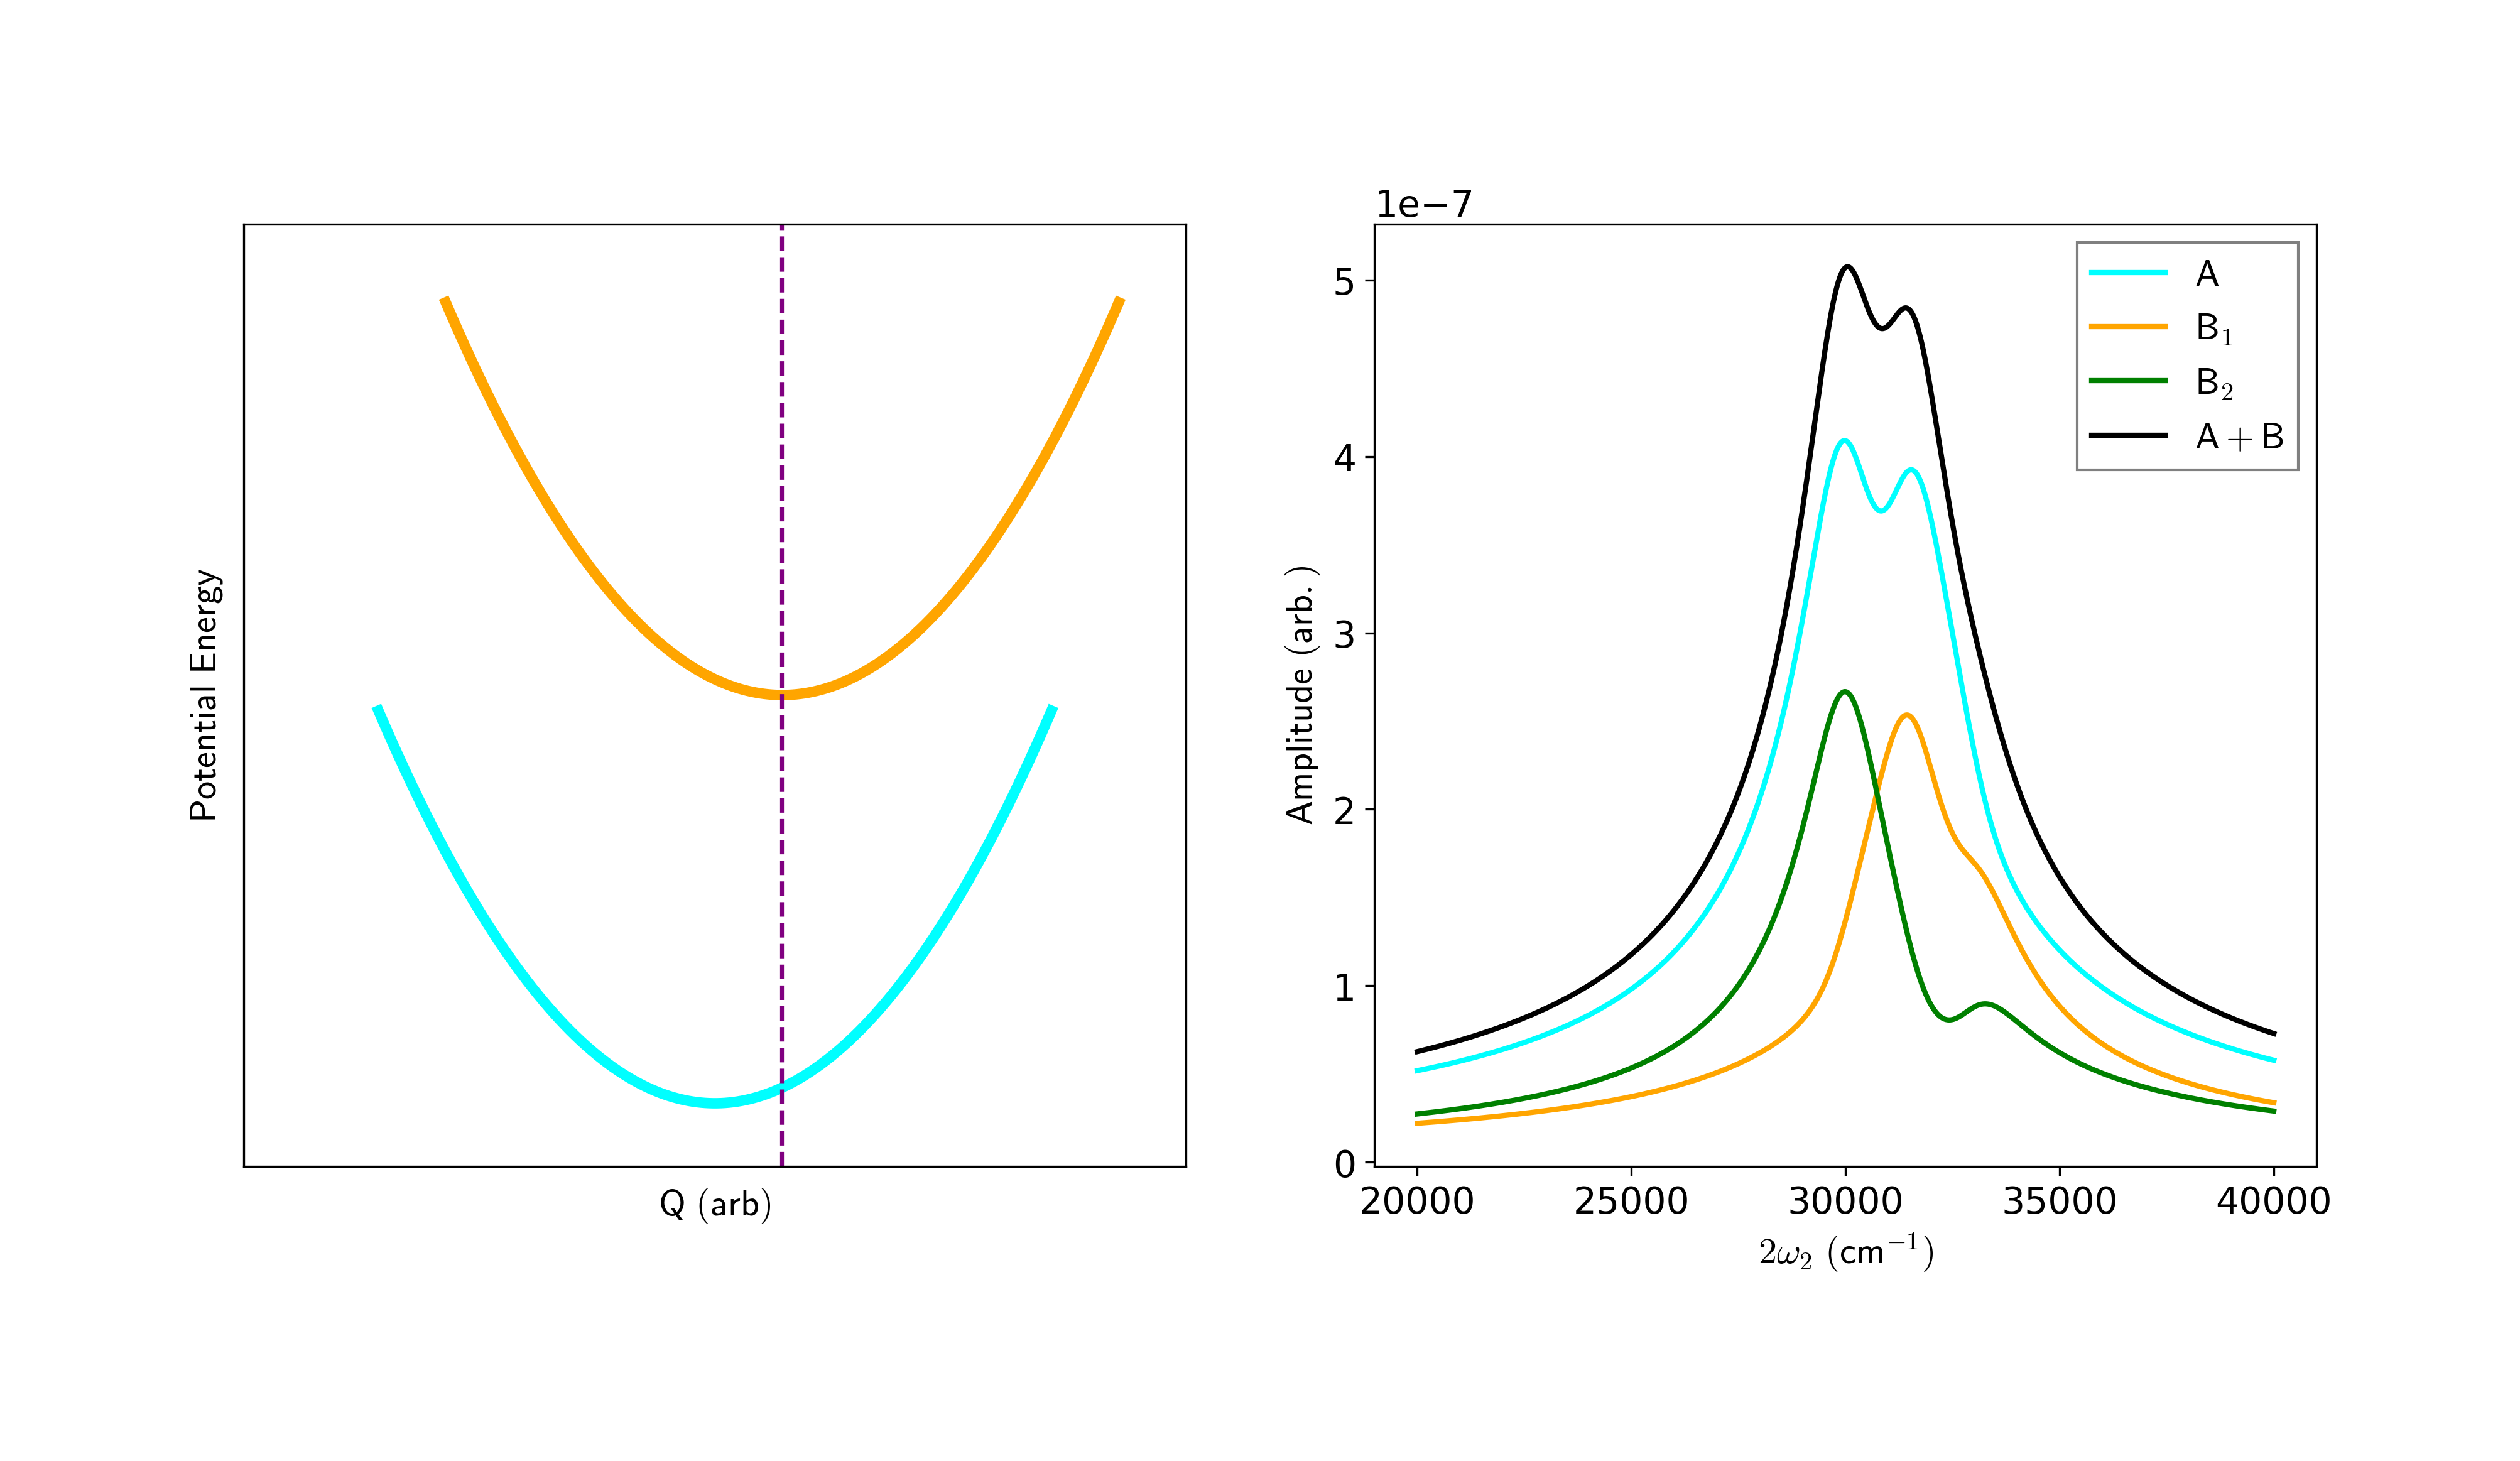
\includegraphics[width=3.375in]{drsive_spectrum.png}
	\caption{Spectrum showing sensitivity of DR-HDFG to well displacements in vibronic coupling.
		Model includes both Franck-Condon and Herzberg Teller effects.
		(a) Potential energy surfaces, 2D spectrum where (b) $\Delta = 0$, (c) $\Delta = 0.5$, (d) $\Delta = 1$}
	\label{fig:doubres_spec}
\end{figure}

%These results also make DR-HDFG a type of resonance IR spectroscopy, as introduced by Boyle et al for resonant triple sum frequency generation.\cite{RN491} 
%However, in the methods described by \autoref{drgamma_alpha_0}, $|e)$ must be accessible through one and two photon transitions from $|g)$.
%Conversely, the resonance-IR method demonstrated by Boyle et al. only requires one photon transitions between $|g)$ and $|e)$.
%Systems which provide strict parity selection rules (e.g., benzene) will be useful for assessing the validity of these selection rules and comparing the method described here and that of Boyle et al. \cite{RN491}

\section{Quantitative Aspects of HDFG}\label{quant}

Since the hyper-Raman process is stimulated by a two-photon process, a setup using only one optical parametric amplifier can perform a coherent four wave mixing hyper-Raman experiment by investigating $\pm \vec{k}_1 + 2\vec{k}_2$ processes (i.e. two laser CMDS), assuming a two photon absorption from a single pulse stimulates the hyper-Raman process.
The most commonly used two laser CMDS method is sum frequency generation, a $\chi^{(2)}$ technique whose phasematching is dictated by $\vec{k}_1 + \vec{k}_2$.
SFG output scales as $\chi^{(2)}_{IJK} \sim \langle \alpha_{ij} \mu_k \rangle$, where $\alpha_{ij}$ is the Raman polarizability tensor.
Since SFG is dependent upon transitions that transform like both rank-one and rank-two tensors, parity enforces a microscopic constraint that SFG cannot yield output for centrosymmetric species under the electric dipole approximation due to the presence of an inversion center. \cite{RN230}
Macroscopically, oddness in spatial inversion of the output polarization eliminates output from centrosymmetric species under the electric dipole approximation.\cite{RN133, RN132}
As a result, the output of SFG is significantly reduced relative to most third order spectroscopies because the output depends on surface species.
However, since HDFG is dependent upon a hyper-Raman transition, it is useful to compare the relative output of the two processes to identify how HDFG output compares to SFG.

To motivate the application of HDFG spectroscopy, we perform a calculation to compare HDFG and vibrational SFG (vSFG) output.
Absorption effects are neglected for simplicity.
The output polarizations of each process is written as
\begin{widetext}
	\begin{subequations}
	\begin{equation}
		\abs{P^{(2)}_{\text{SFG}}} = N_{surf} F(\omega_1+\omega_2) \abs{\langle \alpha_{ij}\mu_{k} \rangle E(\omega_2)E(\omega_1)} 
	\end{equation}
	\begin{equation}
		\abs{P^{(3)}_{\text{HDFG}}} = N_{bulk}  F(2\omega_2-\omega_1) \abs{\langle \beta_{ijk} \mu_{l} \rangle E{(\omega_2)}E(\omega_2)E(-\omega_1)} \ell_{eff}
	\end{equation}
\end{subequations}
\end{widetext}
where N$_{bulk}$ is the bulk number density, and N$_{surf}$ is the surface number density (10$^{19}$ m$^{-2}$).\cite{RN133, RN503}	
For liquids with molar masses less than $\sim$100 g mol$^{-1}$ and densities roughly equal to that of H$_2$O$_{(l)}$ at room temperature, N$_{bulk} \sim$ 10$^{28}$ m$^{-3}$.
We take the bulk optical interaction length ($\ell_{eff}$) to be 10 $\mu$m.\cite{RN133} %see chapter 25 of Shen's NLO book... idk something here seems wrong
A normal dispersion curve is assumed so that $F(\omega_1+\omega_2) \approx F(2\omega_2-\omega_1)$.
To simplify analysis, orientational averaging is ignored (e.g., $\langle \beta_{ijk} \mu_{l} \rangle \approx \beta \mu$) and the input and output fields are taken to be co-polarized, so that
\begin{equation}
		P_{ratio} \equiv \frac{\abs{P^{(3)}_{\text{HDFG}}}}{\abs{P^{(2)}_{\text{SFG}}}} \approx \frac{N_{bulk}}{N_{surf}} \frac{\beta}{\alpha} E(\omega_2) \ell_{eff} \sim 10^4 \frac{\beta}{\alpha} E(\omega_2)\\
\end{equation}
Ziegler has noted that for a field of intensity 10 GW/cm$^{2}$, $\frac{\beta E}{\alpha} \sim 10^{-3} $ for vibrational modes when $E(\omega_2)$ is largely detuned from electronic resonances. \cite{RN515}
Such an intensity is easily obtained using modern ultrafast sources.
In this limit, $P_\text{ratio} \sim 10$.
Since the intensity ratio scales as $\abs{P_{ratio}}^2$, we see that the HDFG output is somewhat stronger than vibrational SFG, assuming only interfacial contributions in vSFG.
It is important to note that this derivation ignored absorption and orientational averaging effects, which can significantly reduce output from either process. 

With the selection rules of HDFG understood for vibrational spectroscopy, it becomes possible to extract quantitative information from its spectra.
Lineshape analysis is essential for extracting quantitative information from CMDS spectra.
Scanning across resonances create dispersive lineshapes, i.e, self-heterodyning, which inform on $\Re(\chi^{(3)})$ and $\Im(\chi^{(3)})$.\cite{Levenson1974_1, Levenson1974_2}
In the method introduced by Levenson and Bloembergen (Bloembergen Interferometry Experiment), an internal standard interferes with the resonant lineshape.
Self-heterodyning of the internal standard signal measures $\chi^{(3)}$ and does not require measurement of absolute intensities. 
Resonant lineshapes are also complicated by amplitude level interference between the sample and its substrate and/or sample cell windows, which must be accounted for to obtain quantitatively correct $\chi^{(3)}$ values. \cite{RN362, RN418}

Most quantitative methods in an n$^{th}$ order CMDS experiment are used to extract $\chi^{(n)}$ values to compare the relative strength of nonlinear processes in different media. \cite{Zhu87, RN351, RN345}
The recorded $\chi^{(n)}$ values provide insight into how microscopic quantities ($\vec{\mu}, \alpha_{ij}, \beta_{ijk}$) impact nonlinear output.
Calculating $\beta_{ijk}$ values from hyper-Raman experiments is difficult and has only been performed for a selection of molecular vibrations. \cite{Xu1997, Shoute2005, Kelley2010}
Methods reported in the literature to measure absolute hyper-Raman polarizabilities depend upon external standards such as hyperpolarizabilities of dissolved samples or two-photon absorption cross sections (also difficult to measure).
Since the Bloembergen interferometry experiment only relies on the third order susceptibility for measured species (such as benzene or CaF$_2$), it is possible to use quantitative four wave mixing spectroscopy to calculcate $\beta_{ijk}$ values.
It is thus useful to investigate how a treatment of orientational averaging can extract $\beta_{ijk}$ from $\chi^{(3)}_{IJKL}$.

The HDFG $\chi^{(3)}_{IJKL}$ expression is
\begin{equation}\label{chi3}
\begin{split}
		\chi^{(3)}_{IJKL} &= NF(\omega_4) \langle \gamma_{ijkl} \rangle = -\frac{NF}{24 \hbar \varepsilon_0 \Delta_{gv}} \langle \beta_{ijk} \mu_l \rangle \rho_{gg}\\
\end{split}
\end{equation}
\autoref{chi3} cannot be used as written to extract $\beta_{ijk}$, as $\beta_{ijk}$ is a Hermitian operator, but $\Delta_{gv} \in \mathbb{C}$. 
However, since the real and imaginary components of $\chi^{(3)}$ can be measured through the Bloembergen interferometry experiment, and $\beta_{ijk}$ is present in either term, we can choose to focus on the real or imaginary part of $\chi^{(3)}$.
For simplicity, we investigate $\Im(\chi^{(3)})$, giving, assuming resonance conditions, 
\begin{equation}
	\langle \beta_{ijk} \mu_{l} \rangle = \frac{24 \hbar \varepsilon_0}{NF} \Gamma_{gv} \frac{1}{\rho_{gg}} \Im(\chi^{(3)}_{IJKL})
\end{equation}
The steps behind orientational averaging of $\gamma_{ijkl}$, a rank four tensor in the molecular frame, are detailed elsewhere.\cite{Andrews1977, McDonnell2024}
Briefly, a tensor in the molecular frame, A$_{ijkl}$ is transformed into an element of the same tensor in the laboratory frame, A$_{IJKL}$ through A$_{IJKL}$ = $\theta^{ijkl}_{IJKL} A_{ijkl} = \langle A_{ijkl} \rangle$, where summation over repeated indices is implied, and $\theta$ is the transformation operator. \cite{McDonnell2024}
Orientational averaging shows specific polarization schemes isolate linear combinations of different $\beta_{ijk}$ terms. \cite{Cyvin1965, Bersohn1966, Kauranen1996}
By introducing the reduced mass coordinate $q_n = \sqrt{\frac{1}{m_n}} Q_n$ and using the expansions of $\beta_{ijk}$ and $\mu_{l}$ to $\order{Q_n}$ found earlier, we see
\begin{equation}\label{betasive}
	\langle \frac{\partial \beta_{ijk}}{\partial q_n} {\frac{\partial \mu_l}{\partial q_n}} \rangle = \frac{48 \varepsilon_0}{NF}  \frac{\Gamma_{gv} \omega_{vg}}{\rho_{gg}} {\Im(\chi^{(3)}_{IJKL})}
\end{equation}
Since $\abs{\mu}$ values can be readily extracted from FT-IR spectra,\cite{RN119, RN412} HDFG can give quantitative information on the magnitude of $\beta_{ijk}$.

\section{Mixed-Domain HDFG}\label{mixeddomain}
The properties of steady state HDFG (complete pulse overlap) are useful for understanding the selection rules that drive output.
Time domain HDFG could be a useful alternative technique for measuring single quantum coherence dephasing times (T$_2$).
The response function for the HDFG pathway illustrated in \autoref{fig:hdfg}a, assuming $\omega_2$ and $\omega_3$ are temporally overlapped, is \cite{RN287, Cho2001}
\begin{equation}
	R^{(3)}(t) = \frac{i}{\hbar} [\beta(t), \mu(0)] \exp(-i\Delta_{gv}t) \theta(t) 
\end{equation}  
The pure time-domain HDFG output reports on the dephasing characteristics of the $\ket{g}\bra{v}$ coherence. 
This method provides practitioners of sum frequency generation the ability to probe isotropic dephasing dynamics without many meaningful changes in their optical setup, and thus compare $\ket{g}\bra{v}$ dephasing in the bulk and at the interface.\cite{RN224}

Transient HDFG spectroscopy, or pump-HDFG-probe, similar to transient vSFG spectroscopy, can be implemented to learn about relaxation dynamics in isotropic systems. \cite{RN224, Bonn2024}
A useful attribute of the $\beta_{ijk}$ dependence in HDFG output is added polarization control. 
Similar to SFG experiments that probe different elements of the infrared transition dipole and Raman polarizability tensors, probing different elements of $\beta_{ijk}$ in HDFG can greatly assist in understanding ultrafast dynamics in isotropic systems, as suggested by Seliya et al. \cite{Shen90, RN224, Bonn2024}
Polarization control in IR-pump-HDFG-probe, analogous to ultrafast transient absorption spectroscopy for vibrational modes, would be an interesting venue to assess the sensitivity of HDFG to different hyper-Raman tensor elements. 

Combinations of time and frequency domain spectroscopy, also called mixed domain spectroscopy, are useful ways to understand frequency-dependent dynamics. \cite{RN135, RN171, RN131}
Mixed domain spectroscopy is a useful alternative to steady state spectroscopy as pulse separation can eliminate nonresonant background and isolate specific pulse ordering sequences. \cite{RN372, RN324, McDonnell2024}
Isolating different pulse orderings can isolate pathway specific signal and minimize interference from unwanted pathways which share the same phasematching constraints. 
Mixed domain HDFG can resolve frequency dependent free induction decay, which could prove useful for understanding isotropic dynamics of single quantum coherences. 
Mixed domain resonant HDFG, using pathways similar to those in \autoref{fig:hdfg}b, could also measure electronic-vibrational correlation functions, as discussed by Cho. \cite{Cho2001}

It is well known that nonlinear wave mixing processes which share the same time ordering and output frequency will interfere. \cite{RN342, RN135}
Understanding interfering pathways is useful because they can, in some cases, eliminate output. 
While we have only isolated one specific HDFG process so far, there are at least fourteen different WMELs which can provide HDFG output. \cite{RN352}
If $\omega_2$ ($\omega_1$) becomes resonant (non-resonant), then other HDFG pathways appear (\autoref{fig:sivewmel2}).\cite{McDonnell2024} 
While the methods in \autoref{fig:sivewmel2} possess identical selection rules to \autoref{fig:hdfg}, the WMEL diagrams presented in \autoref{fig:sivewmel2} will interfere, as they share the same phasematching condition but have oppositely signed amplitudes.
\begin{figure}[!htbp]
	\centering
	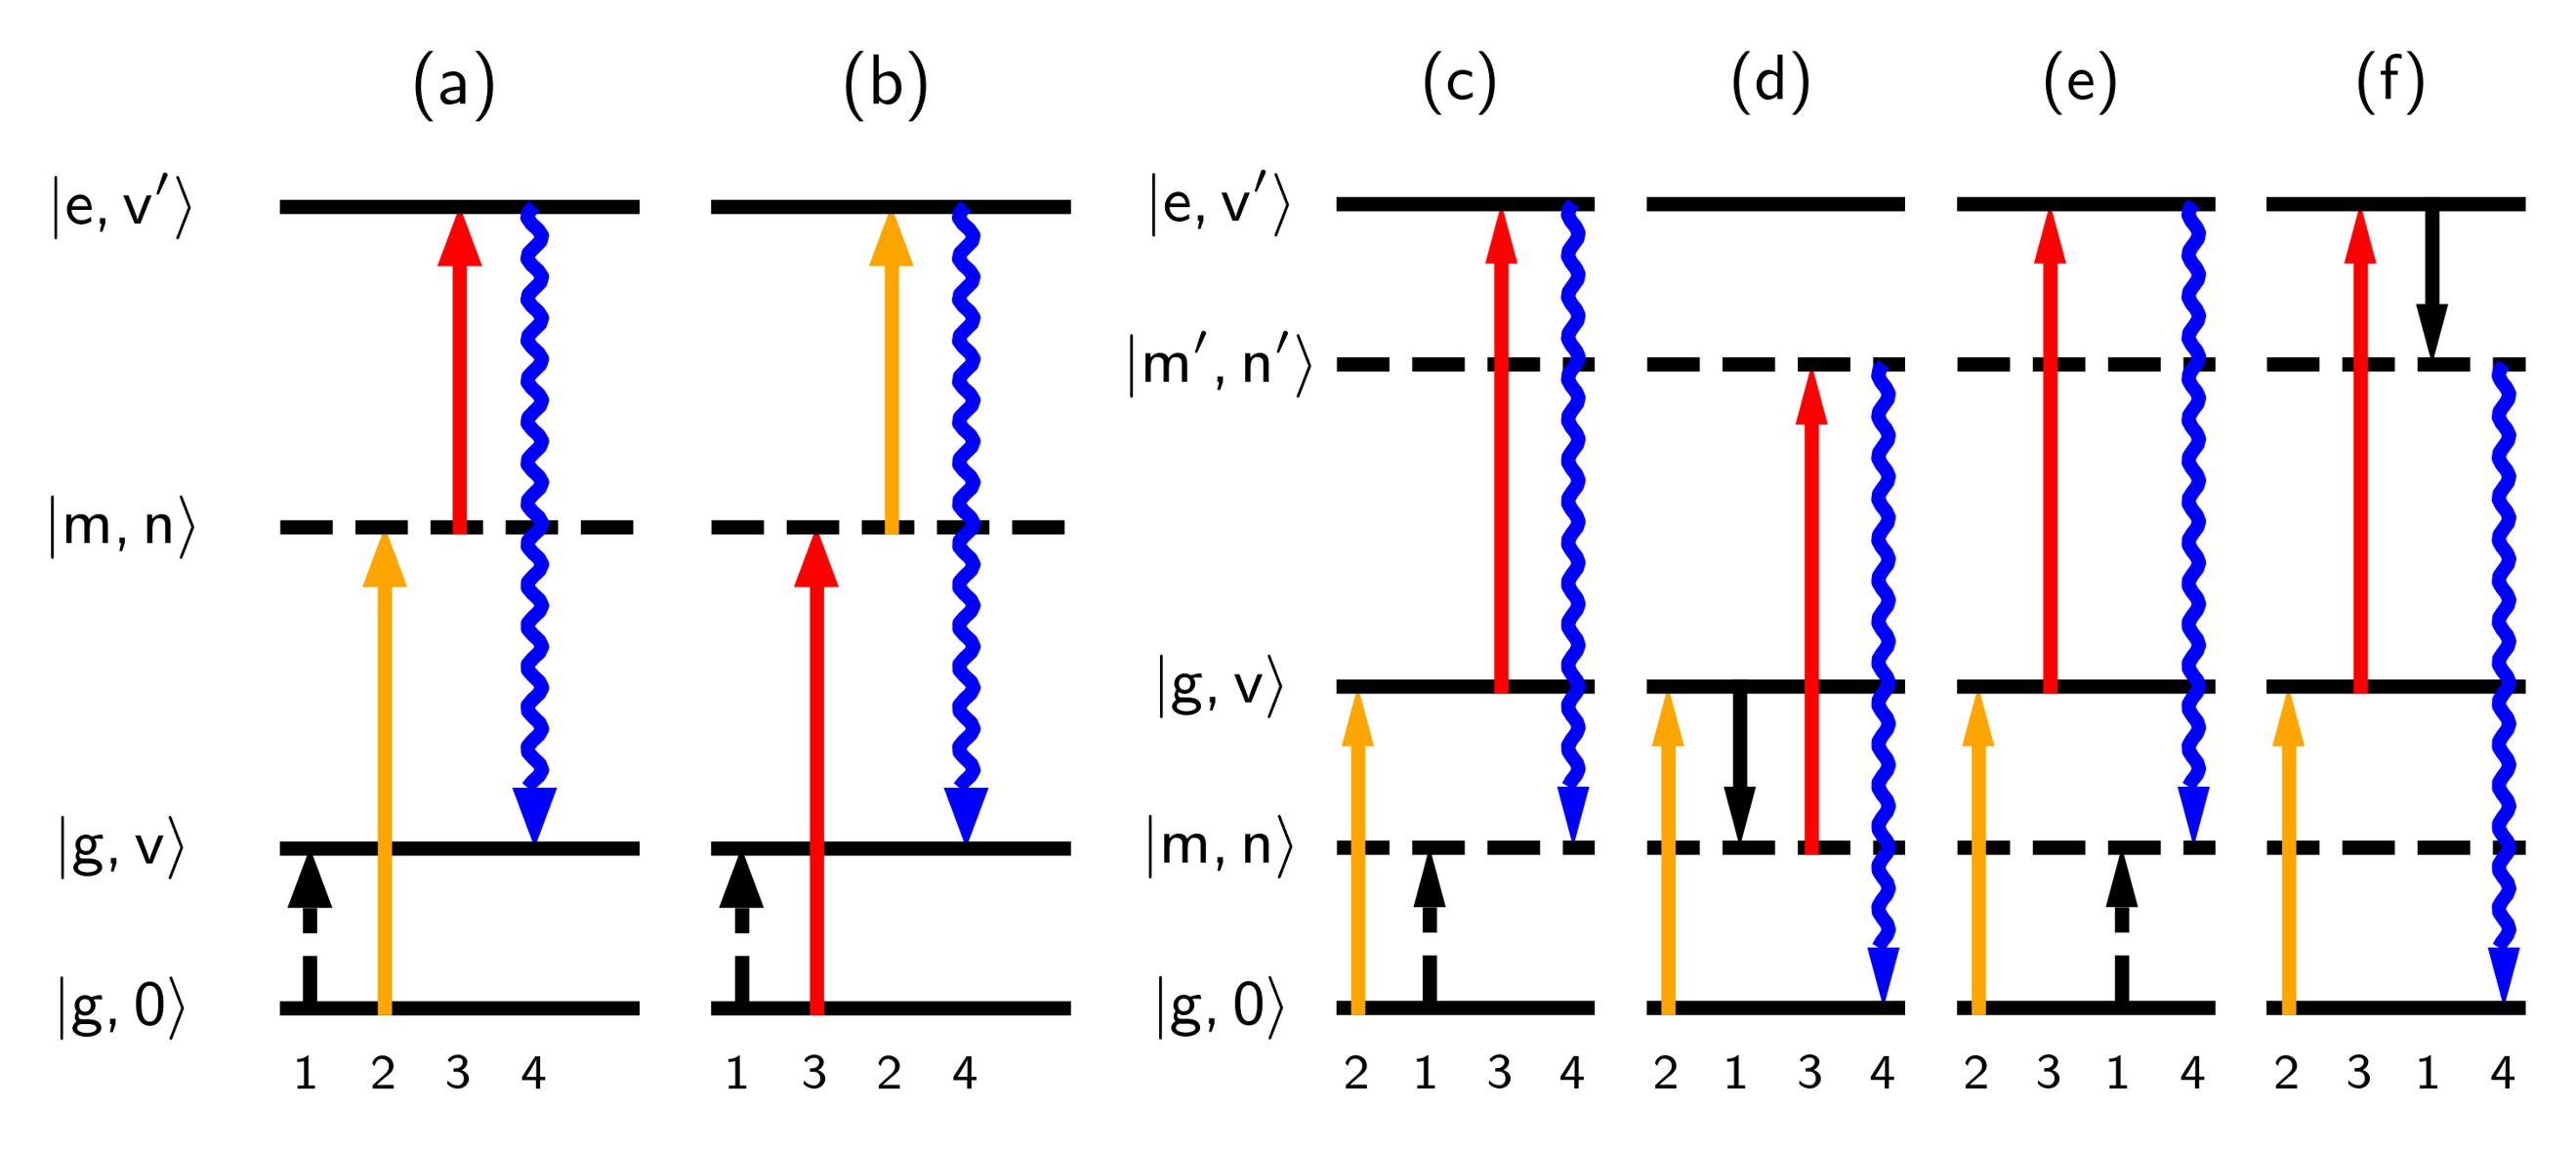
\includegraphics[width=3.375in]{figures/timeorderedwmel.png}
	\caption{WMEL diagrams of interfering HDFG pathways in the  $\vec{k}_4 = -\vec{k}_1 + \vec{k}_2 + \vec{k}_3$ phasematching geometry. 
		}
	\label{fig:sivewmel2}
\end{figure}

The third order response functions for \autoref{fig:sivewmel2}a ($R^{(3)}_{a}$) and \autoref{fig:sivewmel2}b ($R^{(3)}_{b}$) are 
\begin{subequations}
	\begin{equation} \label{mixing:a}
		R^{(3)}_{a} (t_2) = -\frac{i}{\hbar} [\beta(t_2), \mu(0)] \exp(-i\Delta_{v''g}t_2) \theta(t_2)
	\end{equation}
	\begin{equation}\label{mixing:b}
		\begin{split}
			R^{(3)}_{b} (t_2) & = \frac{i}{\hbar} [\beta(t_2), \mu(0)] \exp(-i\Delta_{v''g}t_2) \theta(t_2)\\
		\end{split}
	\end{equation}
\end{subequations}
The total response function in this time ordering is therefore $R^{(3)}_\text{tot} (t_2) = R^{(3)}_{a} (t_2) + R^{(3)}_{b} (t_2) = 0$. 
Since the total output response function vanishes in this time-ordering, the pathways in \autoref{fig:sivewmel2} perfectly destructively interfere.
Therefore, to measure dynamics via HDFG, the time ordering shown in \autoref{fig:hdfg} should be used.
These ideas have been seen experimentally in ultrafast DOVE work. \cite{RN367, McDonnell2024}
In the case of the \autoref{fig:hdfg}a time ordering, there are no opportunities for interference from other third order processes. 
However, a possible mechanism for interfering output in the \autoref{fig:hdfg}a pathway is a cascaded second order process (SFG, DFG). \cite{RN243, RN300}
While unimportant in isotropic systems, second order cascades may become important in media where SFG and DFG are allowed, e.g. surfaces or noncentrosymmetric media. 


\section{Experimental HDFG of CH$_3$CN}\label{Expt}
With the theoretical description of HDFG provided, we will investigate steady state and transient HDFG spectra of $\nu$(CH) modes in CH$_3$CN. 


todo: collect Wigner of ch3cn @ caf2. 


\section{Conclusions}%todo:fix!
Coherent vibrational, hyper-Raman coherent four wave mixing spectroscopies are identified and discussed.
Singly resonant SIVE (SR-SIVE) processes are shown to be the coherent hyper-Raman analogue of infrared active vibrations.
Since SR-SIVE is always non-zero for IR active vibrations, the method could be used as an analytical method to optically upconvert infrared transitions with small transition dipoles.
A method for measuring hyper-Raman polarizabilities, $\beta_{ijk}$, through SIVE spectroscopy was identified and discussed.
Extracting the magnitude and sign of $\beta_{ijk}$ using SIVE methods can help assess the quality of theoretical methods which calculate hyper-Raman spectra. 


\section{Acknowledgments}
This work received support from the Department of Energy, Office of Basic Energy Sciences, Division of Materials Sciences and Engineering (Grant no. DE-SC0002162).
R.P.M. acknowledges support from the NSF Graduate Research Fellowship Program (Grant no. DGE-2137424). 


\section{References}
% Create the reference section using BibTeX:
\bibliography{library.bib}

\end{document}
%


